\section{{VISÃO COMPUTACIONAL}}

A visão computacional abrange todas as técnicas e métodos de processamento de imagem em um único meio, com o objetivo de ser mais eficiente nas análises de dados e informações compostas dentro de uma imagem. \citeonline{SILVA2017} contextualizam que algoritmos de visão computacional utiliza matrizes bidimensionais ou hiperdimensionais como entrada de dados e, a partir desta, produzem informações compactadas como saída.

De forma didática, a área de visão computacional utiliza modelos descritivos de objetos, pessoas e/ou cenas capturadas digitalmente para realizar tomadas de decisões, a fim de automatizar processos.

Segundo \citeonline{REHEM2009}, devido ao avanço tecnológico, desenvolveram-se computadores com maior capacidade de processamento gráfico, proporcionando ferramentas com um potencial maior na área de visão computacional. Pode-se dizer que essas ferramentas são bibliotecas onde o seu código fonte é constituído de um agrupamento de funções que potencializam o processamento gráfico de imagens e vídeos. Sendo assim, ao utilizar essas bibliotecas, tem-se a possibilidade de desenvolvimento de técnicas de aperfeiçoamento gráfico para realizar rastreamento de movimentos e de características humanas em tempo real.

Contudo, a visão computacional foi desenvolvida, segundo \citeonline{MARR76}, através da neurofisiologia da visão humana. Seu modelo era estabelecido em níveis de compreensões necessárias à computação da visão estereoscópica, ou seja, o modelo é capaz de trabalhar com eficiência no ambiente tridimensional, onde a análise é feita através de duas imagens obtidas em postos diferentes. \citeonline{PERONTI2008} explica em seu artigo que estereoscopia é a visualização de feita por dois mecanismos de captura de imagem em um mesmo foco.

%\clearpage

\begin{figure}[!htb]
\caption{{\footnotesize Mecanismos para captação de imagens com focos visuais coincidentes.}}
 
\centering % para centralizarmos a figura
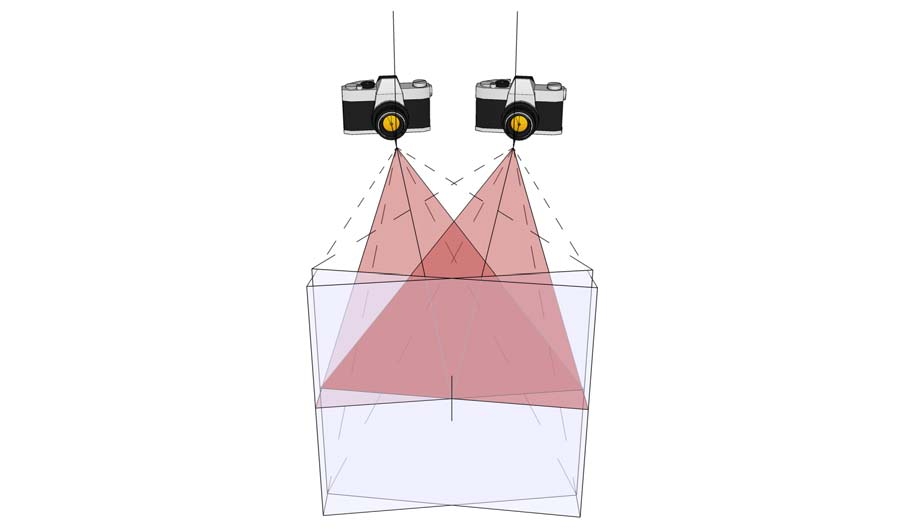
\includegraphics[width=13cm]{revisao-bibliografica/Figuras/visaocamera.png}% leia abaixo
\label{figura:figura9}

\centering \subfloat {\footnotesize { Fonte: \cite{PERONTI2008} }}
{
\label{figura:figura9}
}
\end{figure}

%\clearpage

\begin{figure}[!htb]
\caption{{\footnotesize Esquema mostrando as imagens captadas em cada olho (par estereoscópico) e a imagem resultado da fusão deste par estereoscópico \cite{PERONTI2008}.}}
 
\centering % para centralizarmos a figura
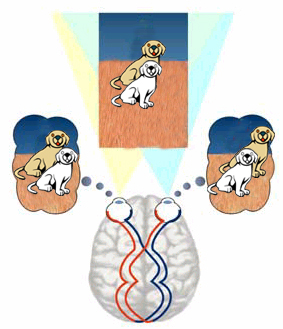
\includegraphics[width=7cm]{revisao-bibliografica/Figuras/visaohumana1.jpg}% leia abaixo
\label{figura:figura10}

\centering \subfloat {\footnotesize { Disponível em: https://i.imgur.com/Mg7u9eF.jpg }}
{
\label{figura:figura10}
}
\end{figure}